%%%%%%%%%%%%%%%%%%%%%%%%%%%%%%%%%%%%%%%%%
% Short Sectioned Assignment
% LaTeX Template
% Version 1.0 (5/5/12)
%
% This template has been downloaded from:
% http://www.LaTeXTemplates.com
%
% Original author:
% Frits Wenneker (http://www.howtotex.com)
%
% License:
% CC BY-NC-SA 3.0 (http://creativecommons.org/licenses/by-nc-sa/3.0/)
%
%%%%%%%%%%%%%%%%%%%%%%%%%%%%%%%%%%%%%%%%%

%----------------------------------------------------------------------------------------
%	PACKAGES AND OTHER DOCUMENT CONFIGURATIONS
%----------------------------------------------------------------------------------------

\documentclass[paper=a4, fontsize=11pt]{scrartcl} % A4 paper and 11pt font size

\usepackage[T1]{fontenc} % Use 8-bit encoding that has 256 glyphs
%\usepackage{fourier} % Use the Adobe Utopia font for the document - comment this line to return to the LaTeX default
\usepackage[english]{babel} % English language/hyphenation
\usepackage{amsmath,amsfonts,amsthm} % Math packages

\usepackage{lipsum} % Used for inserting dummy 'Lorem ipsum' text into the template

\usepackage{graphicx}
\usepackage{caption}
\usepackage{subcaption}

\usepackage{sectsty} % Allows customizing section commands
\allsectionsfont{\centering \normalfont\scshape} % Make all sections centered, the default font and small caps

\usepackage{fancyhdr} % Custom headers and footers
\pagestyle{fancyplain} % Makes all pages in the document conform to the custom headers and footers
\fancyhead{} % No page header - if you want one, create it in the same way as the footers below
\fancyfoot[L]{} % Empty left footer
\fancyfoot[C]{} % Empty center footer
\fancyfoot[R]{\thepage} % Page numbering for right footer
\renewcommand{\headrulewidth}{0pt} % Remove header underlines
\renewcommand{\footrulewidth}{0pt} % Remove footer underlines
\setlength{\headheight}{13.6pt} % Customize the height of the header

\numberwithin{equation}{section} % Number equations within sections (i.e. 1.1, 1.2, 2.1, 2.2 instead of 1, 2, 3, 4)
\numberwithin{figure}{section} % Number figures within sections (i.e. 1.1, 1.2, 2.1, 2.2 instead of 1, 2, 3, 4)
\numberwithin{table}{section} % Number tables within sections (i.e. 1.1, 1.2, 2.1, 2.2 instead of 1, 2, 3, 4)

\setlength\parindent{0pt} % Removes all indentation from paragraphs - comment this line for an assignment with lots of text

%----------------------------------------------------------------------------------------
%	TITLE SECTION
%----------------------------------------------------------------------------------------

\newcommand{\horrule}[1]{\rule{\linewidth}{#1}} % Create horizontal rule command with 1 argument of height

\title{	
\normalfont \normalsize 
\textsc{ETH Zurich, D-INFK} \\ [25pt] % Your university, school and/or department name(s)
\horrule{0.5pt} \\[0.4cm] % Thin top horizontal rule
\huge Computer Vision: Exercise 12 Tracking \\ % The assignment title
\horrule{2pt} \\[0.5cm] % Thick bottom horizontal rule
}

\author{Igor Pesic} % Your name

\date{\normalsize\today} % Today's date or a custom date

\begin{document}

\maketitle % Print the title


\section{Video 1}

Tracejtories for video 1 are shown in Figure \ref{fig:v1}. 

\begin{figure}
\centering
\begin{subfigure}{.5\textwidth}
  \centering
  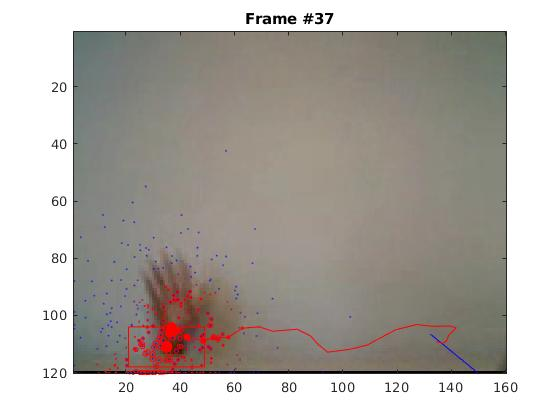
\includegraphics[width=.9\linewidth]{video10.jpg}
  \caption{Model 0}
\end{subfigure}%
\begin{subfigure}{.5\textwidth}
  \centering
  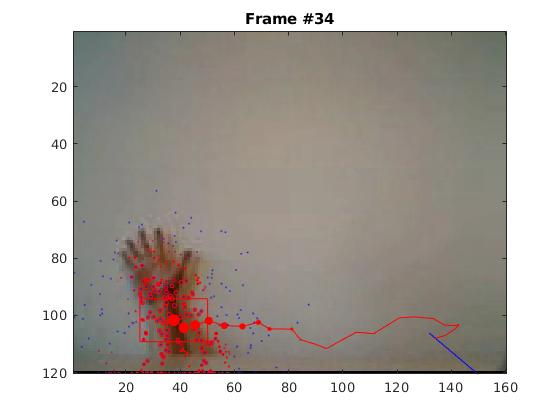
\includegraphics[width=.9\linewidth]{video11.jpg}
  \caption{Model 1}
\end{subfigure}
\caption{Video 1}
\label{fig:v1}x
\end{figure}


\section{Video 2}

Trajectories for video 2 for 2 different types of models (i.e. with and without velocity) are shown in Figure \ref{fig:v2_model}. As we can notice there are no significant changes for the 2 types of models. It can be explained by the slow movement of the object. Because of the slow movement, the noise can capture the moves and thus no significant improvement exists with modeling the speed.

\begin{figure}
\centering
\begin{subfigure}{.5\textwidth}
  \centering
  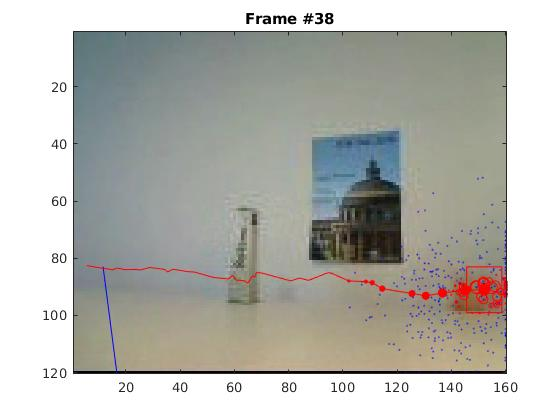
\includegraphics[width=.9\linewidth]{video20.jpg}
  \caption{Model 0}
\end{subfigure}%
\begin{subfigure}{.5\textwidth}
  \centering
  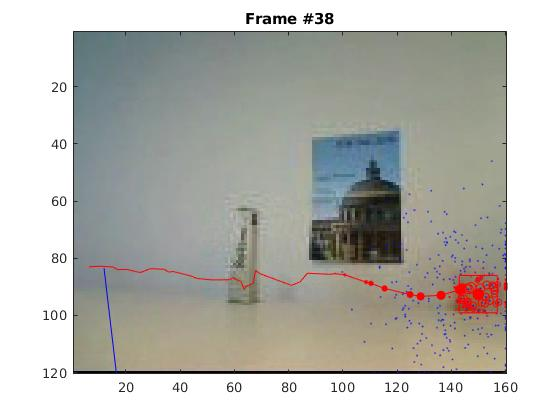
\includegraphics[width=.9\linewidth]{video21.jpg}
  \caption{Model 1}
\end{subfigure}
\caption{Video 2}
\label{fig:v2_model}
\end{figure}

The change of the system noise mostly affects the a-priori distribution of particles (which is expected since it adds more noise to a-priori distribution) and it only slightly affects the a-posteriori distribution and almost has no significant effect on the final result. The Figure \ref{fig:v2_sys_noise} shows these findings.

\begin{figure}
\centering
\begin{subfigure}{.5\textwidth}
  \centering
  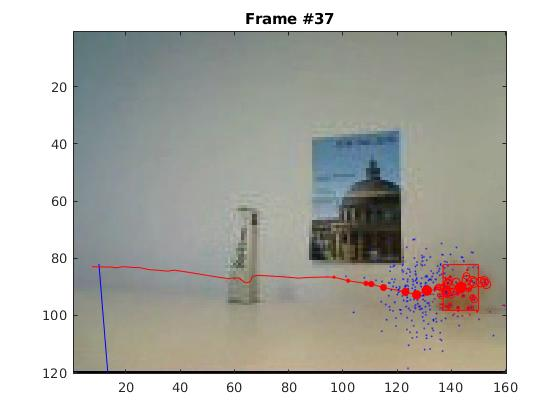
\includegraphics[width=.9\linewidth]{video21_l_sys_sigma.jpg}
  \caption{Low system noise}
\end{subfigure}%
\begin{subfigure}{.5\textwidth}
  \centering
  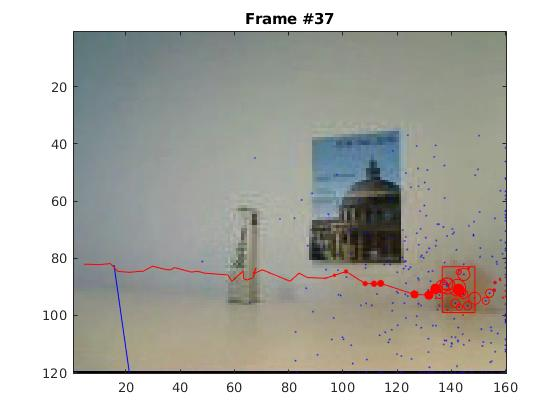
\includegraphics[width=.9\linewidth]{video21_h_sys_sigma.jpg}
  \caption{High system noise}
\end{subfigure}
\caption{Video 2}
\label{fig:v2_sys_noise}
\end{figure}

The change of the observation noise mostly affects the a-posteriori distribution of particles since the algorithm more often samples from the outlying particles when the observation noise is larger. The results are shown in Figure \ref{fig:v2_obs_noise}.

\begin{figure}
\centering
\begin{subfigure}{.5\textwidth}
  \centering
  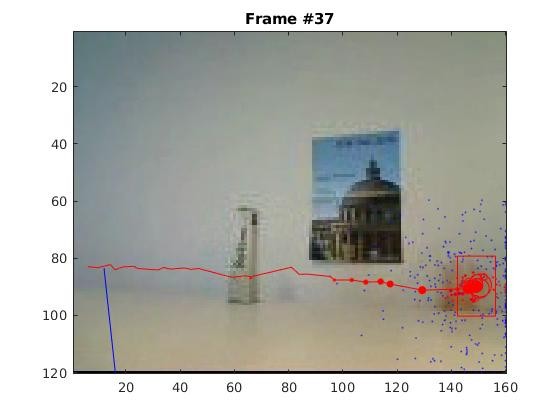
\includegraphics[width=.9\linewidth]{video21_l_obs_sigma.jpg}
  \caption{Low observation noise}
\end{subfigure}%
\begin{subfigure}{.5\textwidth}
  \centering
  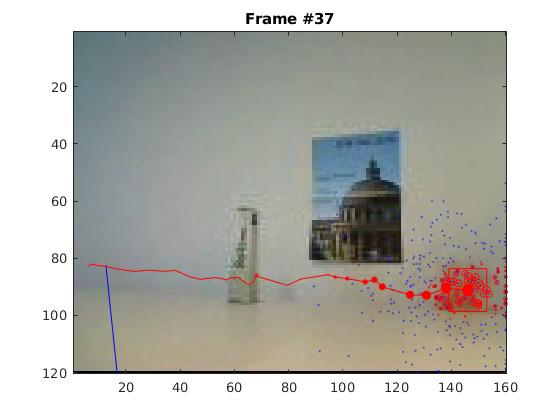
\includegraphics[width=.9\linewidth]{video21_h_obs_sigma.jpg}
  \caption{High observation noise}
\end{subfigure}
\caption{Video 2}
\label{fig:v2_obs_noise}
\end{figure}

\section{Video 3}

After trying the different values for the parameters from part 2, I have discovered that high system noise brings very poor results and very low system noise sometimes fails to track the fast movements of the ball. Also high measurements noise fails because it loses the track of ball and starts tracking the edge of the table on the right part of the frame. Both types of models (no velocity and constant velocity) performed well on the 3th video. The trajectory obtained with the best parameters is shown in Figure \ref{fig:v3}.

\begin{figure}
  \centering
  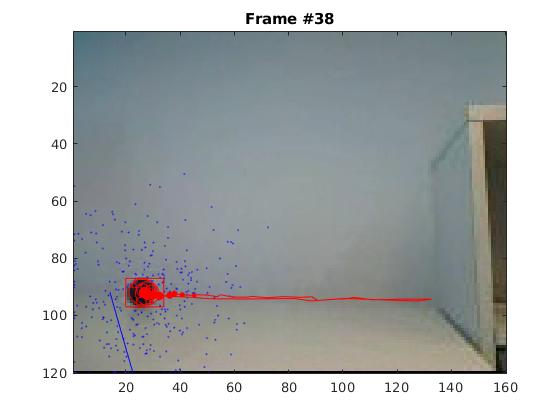
\includegraphics[width=.9\linewidth]{video3.jpg}


\caption{Video 3}
\label{fig:v3}
\end{figure}


\section{Conclusion}

Finally I have tested the effect of number of particles and as expected, I have observed that too few particles (e.g. 50) brings very poor results, and more particles (e.g. 500) shows very good results. This can be explained by the fact that we work with the discrete probability distribution and thus more particles represent the better approximation of the probability distribution.

The similar holds for the number of bins: more bins we have, better we can describe the object and thus better the results.Too few bins fail to track the object (see Figure \ref{fig:v3_f}). Nevertheless, 8 bins was still good enough for these videos.

\begin{figure}
  \centering
  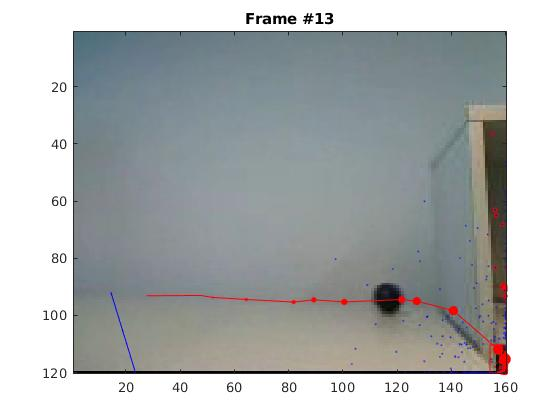
\includegraphics[width=.9\linewidth]{video3_fail.jpg}


\caption{Video 3 Failed}
\label{fig:v3_f}
\end{figure}

\end{document}